
\documentclass[xcolor=pdftex,dvipsnames,table,mathserif,aspectratio=169]{beamer}
\usetheme{default}
\usetheme{metropolis}
\usepackage{mathtools}
\setbeamersize{text margin left=.3in,text margin right=.3in} 

\DeclarePairedDelimiter\abs{\lvert}{\rvert}%
\DeclarePairedDelimiter\norm{\lVert}{\rVert}%


%\usetheme{Darmstadt}
%\usepackage{times}
%\usefonttheme{structurebold}

\usepackage[english]{babel}
%\usepackage[table]{xcolor}
\usepackage{pgf,pgfarrows,pgfnodes,pgfautomata,pgfheaps}
\usepackage{amsmath,amssymb,setspace,centernot}
\usepackage[latin1]{inputenc}
\usepackage[T1]{fontenc}
\usepackage{relsize}
\usepackage{pdfpages}
\usepackage[absolute,overlay]{textpos} 


\newenvironment{reference}[2]{% 
  \begin{textblock*}{\textwidth}(#1,#2) 
      \footnotesize\it\bgroup\color{red!50!black}}{\egroup\end{textblock*}} 

\DeclareMathSizes{10}{10}{6}{6} 

\begin{document}
\title{Part 8: Policy Evaluation (e):\\
 Regression Discontinuity}
\author{Chris Conlon}
\institute{Applied Econometrics}
\date{\today}

\frame{\titlepage}
\begin{frame}{Regression Discontinuity Design}
\begin{itemize}
\item Another popular research design is the \alert{Regression Discontinuity Design}.
\item In some sense this is a special case of IV regression. (RDD estimates a LATE).
\item Most of this is taken from the JEL Paper by Lee and Lemieux (2010).
\end{itemize}              
\end{frame}

\begin{frame}{RDD: Basics}
\begin{itemize}
\item We have a \alert{running or forcing variable} $x$ such that 
\begin{eqnarray*}
\lim_{x\rightarrow c^{+}} P(T_i | X_i = x) \neq \lim_{x\rightarrow c^{-}}P(T_i | X_i = x)
\end{eqnarray*}
\item The idea is that there is a \alert{discontinuous jump} in the \alert{probability of being treated}.
\item For now we focus on the \alert{sharp discontinuity}:\\
 $P(T_i | X_i \geq c) =1$ and $P(T_i | X_i < c) =0$
 \item There is no single $x$ for which we observe treatment and control.\\
  (Compare to Propensity Score!).
\end{itemize}              
\end{frame}


\begin{frame}{RDD: Basics}
\begin{itemize}
\item Example: a social program is available to people who earned less than \$25,000.
\begin{itemize}              
\item If we could compare people earning \$24,999 to people earning \$25,001 we would have as-if random assignment. (MAYBE)
\item But we might not have that many people...
\end{itemize}
\item We are going to label the \alert{treatment effect} $\tau_i$.\\
Note: my lack of precision here!
\item The most important assumption is that of \alert{no manipulability} $\tau_i  \perp T_i$ in some neighborhood of $c$.
\begin{itemize}
\item If agents can \alert{choose} $x_i$ we are in trouble: underreporting income, avoiding ``possession with intent to distribute'' for drugs, etc.
\end{itemize}              
\end{itemize}              
\end{frame}


\begin{frame}{RDD: Continuity}
\begin{itemize}
\item The central idea in RDD is that of \alert{continuity}
\item We need that $E[Y(1)  | X]$ and $E[Y(0) | X]$ both be continuous at $X=c$.
\begin{itemize}
\item We expect that $Y_i = f(x_i)$ to be a smooth, continuous function of $x_i$
\item The \alert{only} departure from that is the treatment $\tau_i \cdot I(x_i \geq c)$.
\end{itemize}
\item We want to be as agnostic as possible about \alert{functional form}
\begin{itemize}
\item Don't want to restrict ourselves to $f(x_i) = \beta_0 + \beta_1 x_i$.
\item The central idea: we know $f(x_i)$ absent the treatment!
\end{itemize}   
\end{itemize}              
\end{frame}


\begin{frame}{RDD: In Pictures}
\begin{center}
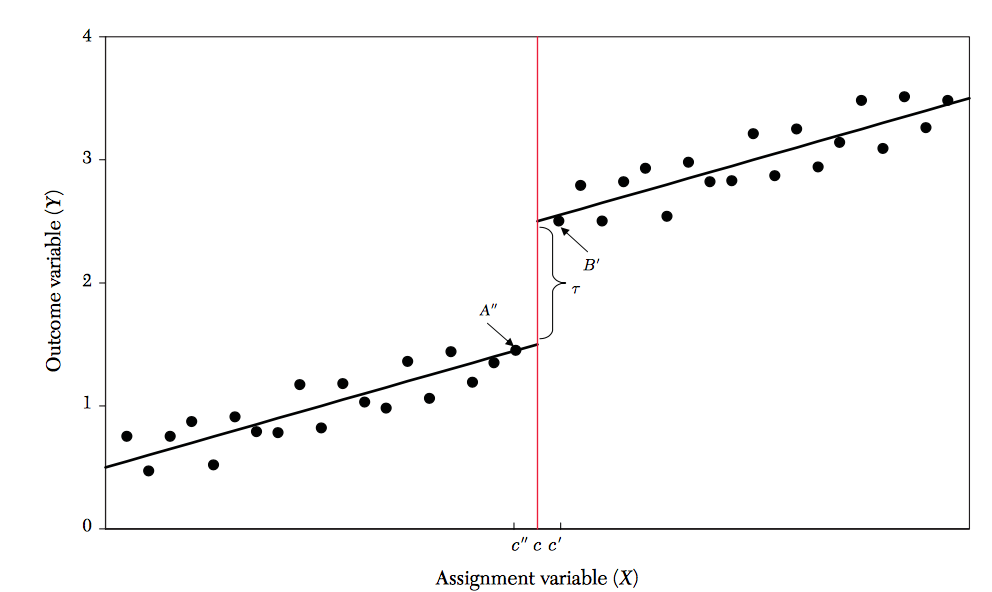
\includegraphics[width=4.5in]{./resources/ll-fig1}
\end{center}
\end{frame}


\begin{frame}{RDD: Sharp RD Case}
RDD uses a set of assumptions distinct from our LATE/IV assumptions. Instead it depends on \alert{continuity}.
\begin{itemize}
\item People just to the left of $c$ are a valid control for those just to the right of $c$.
\item \alert{This is not a testable assumption} $\rightarrow$ draw pictures!
\item We could run the regression where $T_i = \mathbf{1}[X_i > c]$.
\begin{eqnarray*}
Y_i = \beta_0 + \tau_i \cdot T_i + X_i \beta + \epsilon_i
\end{eqnarray*}
\item This puts a lot of restrictions (linearity) on the relationship between $Y$ and $X$.
\item Also (without additional assumptions) we only learn about $\tau_i$ at the point $X=c$.
\end{itemize}
\end{frame}


\begin{frame}{RDD: Nonlinearity}
First thing to relax is assumption of linearity.
\begin{eqnarray*}
Y_i = f(x_i) + \tau T_i  + \epsilon_i
\end{eqnarray*}
This is known as \alert{partially linear model}.
\begin{itemize}
\item Three options for $f(x_i)$:
\begin{enumerate}
\item Kernels
\item Polynomials: $Y_i = \beta_0 + \beta_1 x_i + \beta_2 x_i^2 + \cdots + \beta_p x^p + \tau T_i + \epsilon_i$.
\begin{itemize}
\item Actually, people suggest different polynomials on each side of cutoff! (Interact everything with $T_i$).
\end{itemize}
\item Local Linear/Polynomial Regression
\end{enumerate}
\item Same objective. Want to flexibly capture what happens on both sides of cutoff.
\item Otherwise risk confusing nonlinearity with discontinuity!
\end{itemize}
\end{frame}
	
\begin{frame}{RDD: Kernel Boundary Problem}
\begin{center}
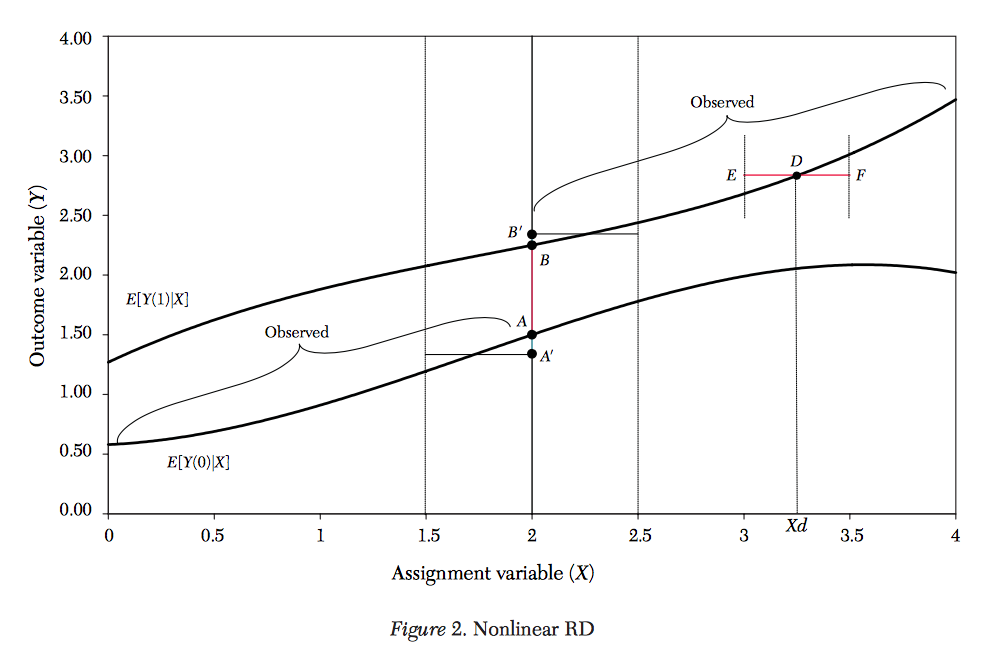
\includegraphics[width=4.5in]{./resources/ll-fig2}
\end{center}
\end{frame}

\begin{frame}{RDD: Polynomial Implementation Details}
To make life easier:
\begin{itemize}
\item replace $\tilde{x}_i = x_i - c$.
\item Estimate coefficients $\beta$: $(1, \tilde{x}, \tilde{x}^2, \ldots, \tilde{x}^p)$ and\\
 $\tilde{\beta}$: $(T_i, T_i \tilde{x},T_i \tilde{x}^2, \ldots, T_i \tilde{x}^p)$.
 \item Now treatment effect at $c$ just the coefficient on $T_i$. (We can ignore the interaction terms).
 \item If we want treatment effect at $x_i > c$ then we have to account for interactions.
 \begin{itemize}
 \item Identification away from $c$ is somewhat dubious anyway.
\end{itemize}
\item Lee and Lemieux (2010) suggest estimating a coefficient on a dummy for each bin in the polynomial regression $\sum_{k} \phi_k B_k$.
 \begin{itemize}
 \item Add polynomials until you can satisfy the test that the joint hypothesis test that $\phi_1 = \cdots \phi_k= 0$.
\item There are better ways to choose polynomial order...
\end{itemize}
\end{itemize}
\end{frame}

	
\begin{frame}{RDD: Checklist}
Most RDD papers follow the same formula (so should yours)
\begin{itemize}
\item Plot of $P(T | X)$ so that we can see the discontinuity
\item Plot of $E[Y | X]$ so that we see discontinuity there also
\item Plot of $E[W | X ]$ so that we don't see a discontinuity in controls.
\item Density of $X$ (check for manipulation).
\item Show robustness to different ``windows''
\item The OLS RDD estimates
\item The Local Linear RDD estimates
\item The polynomial (from each side) RDD estimates
\item An f-test of ``bins'' showing that the polynomial is flexible enough.
\end{itemize}
Read Lee and Lemieux (2010) before you get started.\\
The \texttt{rdd} package in R has many of these features.
\end{frame}


\begin{frame}{Application: Lee (2008)}
Looked at incumbency advantage in the US House of Representatives
\begin{itemize}
\item Running variable was vote share in previous election
\begin{itemize}
\item Problem of naive approach: good candidates get lots of votes!
\item Compare outcomes of districts with barely $D$ to barely $R$.
\end{itemize}
\item First we plot bin-scatter plots and quartic (from each side) polynomials.
\item Discussion about how to choose bin-scatter bandwidth (CV).
\end{itemize}
\end{frame}

\begin{frame}{Lee (2008)}
\begin{center}
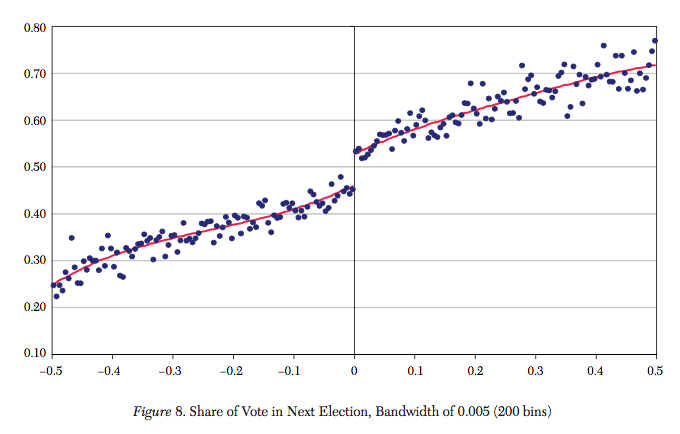
\includegraphics[width=4.5in]{./resources/binscatter1}
\end{center}
\end{frame}

\begin{frame}{Lee (2008)}
\begin{center}
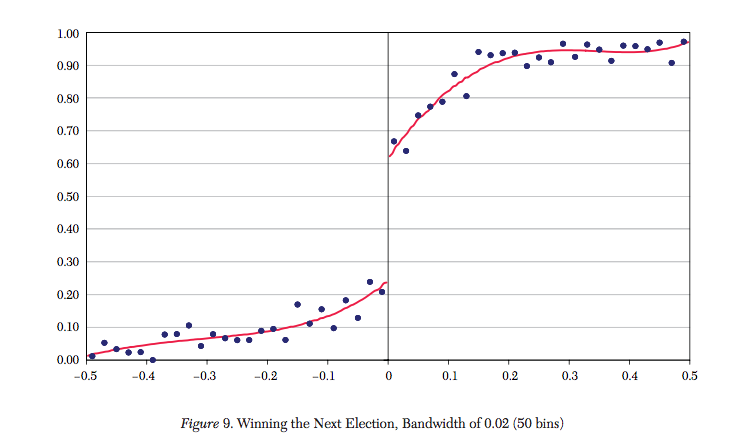
\includegraphics[width=4.5in]{./resources/binscatter2}
\end{center}
\end{frame}

\begin{frame}{Lee (2008)}
\begin{center}
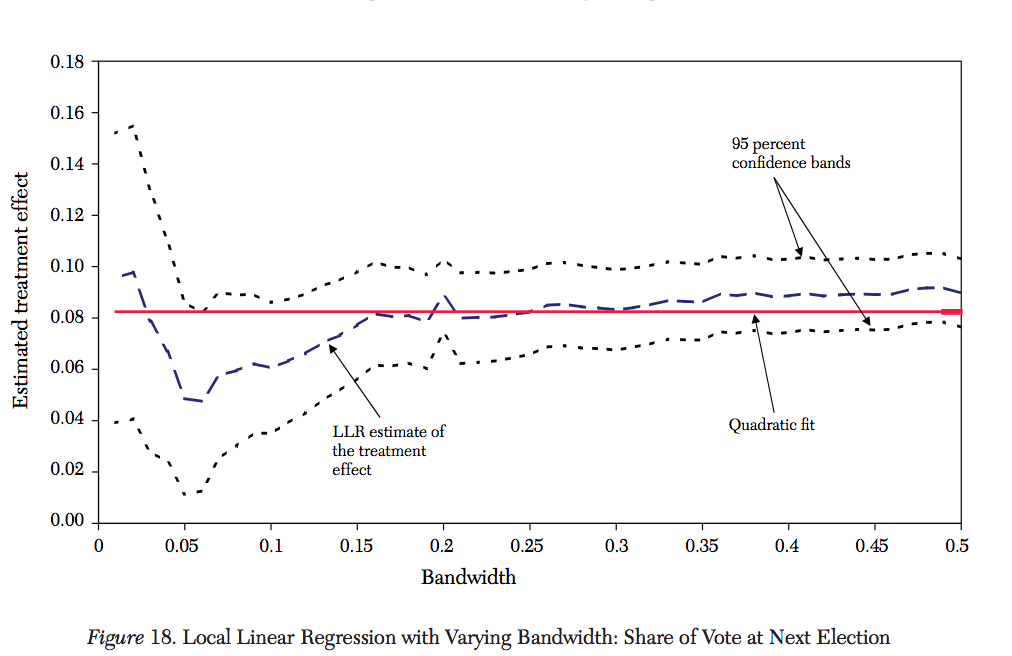
\includegraphics[width=4.5in]{./resources/ll-fig4}
\end{center}
\end{frame}

\begin{frame}{Other Examples}
Luca on Yelp
\begin{itemize}
\item Have data on restaurant revenues and yelp ratings.
\item Yelp produces a yelp score (weighted average rating) to two decimals ie: $4.32$.
\item Score gets rounded to nearest half star
\item Compare $4.24$ to $4.26$ to see the impact of an extra half star.
\item Now there are multiple discontinuities: Pool  them? Estimate multiple effects?
\end{itemize}
\end{frame}

\begin{frame}{Manipulation}
McCrary (2008) develops a test for manipulation in running variable $x$
\begin{center}
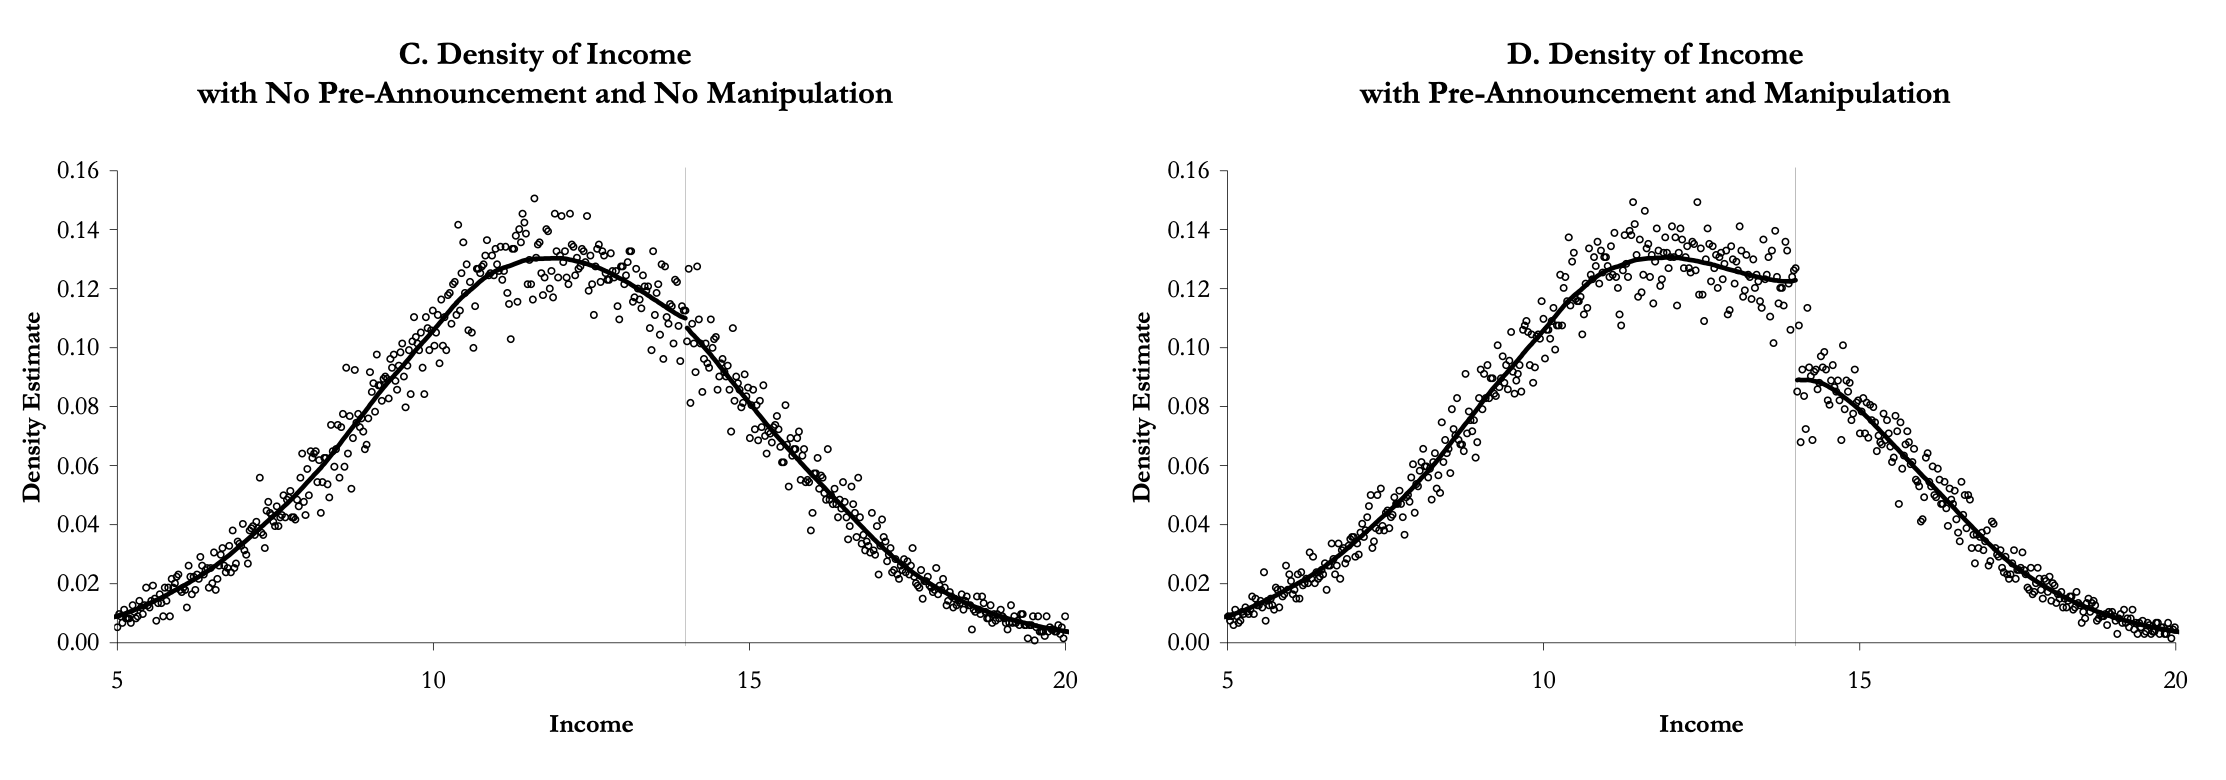
\includegraphics[width=5.75in]{./resources/mccrary1.png}
\end{center}
\end{frame}


\begin{frame}{Manipulation: Good}
\begin{center}
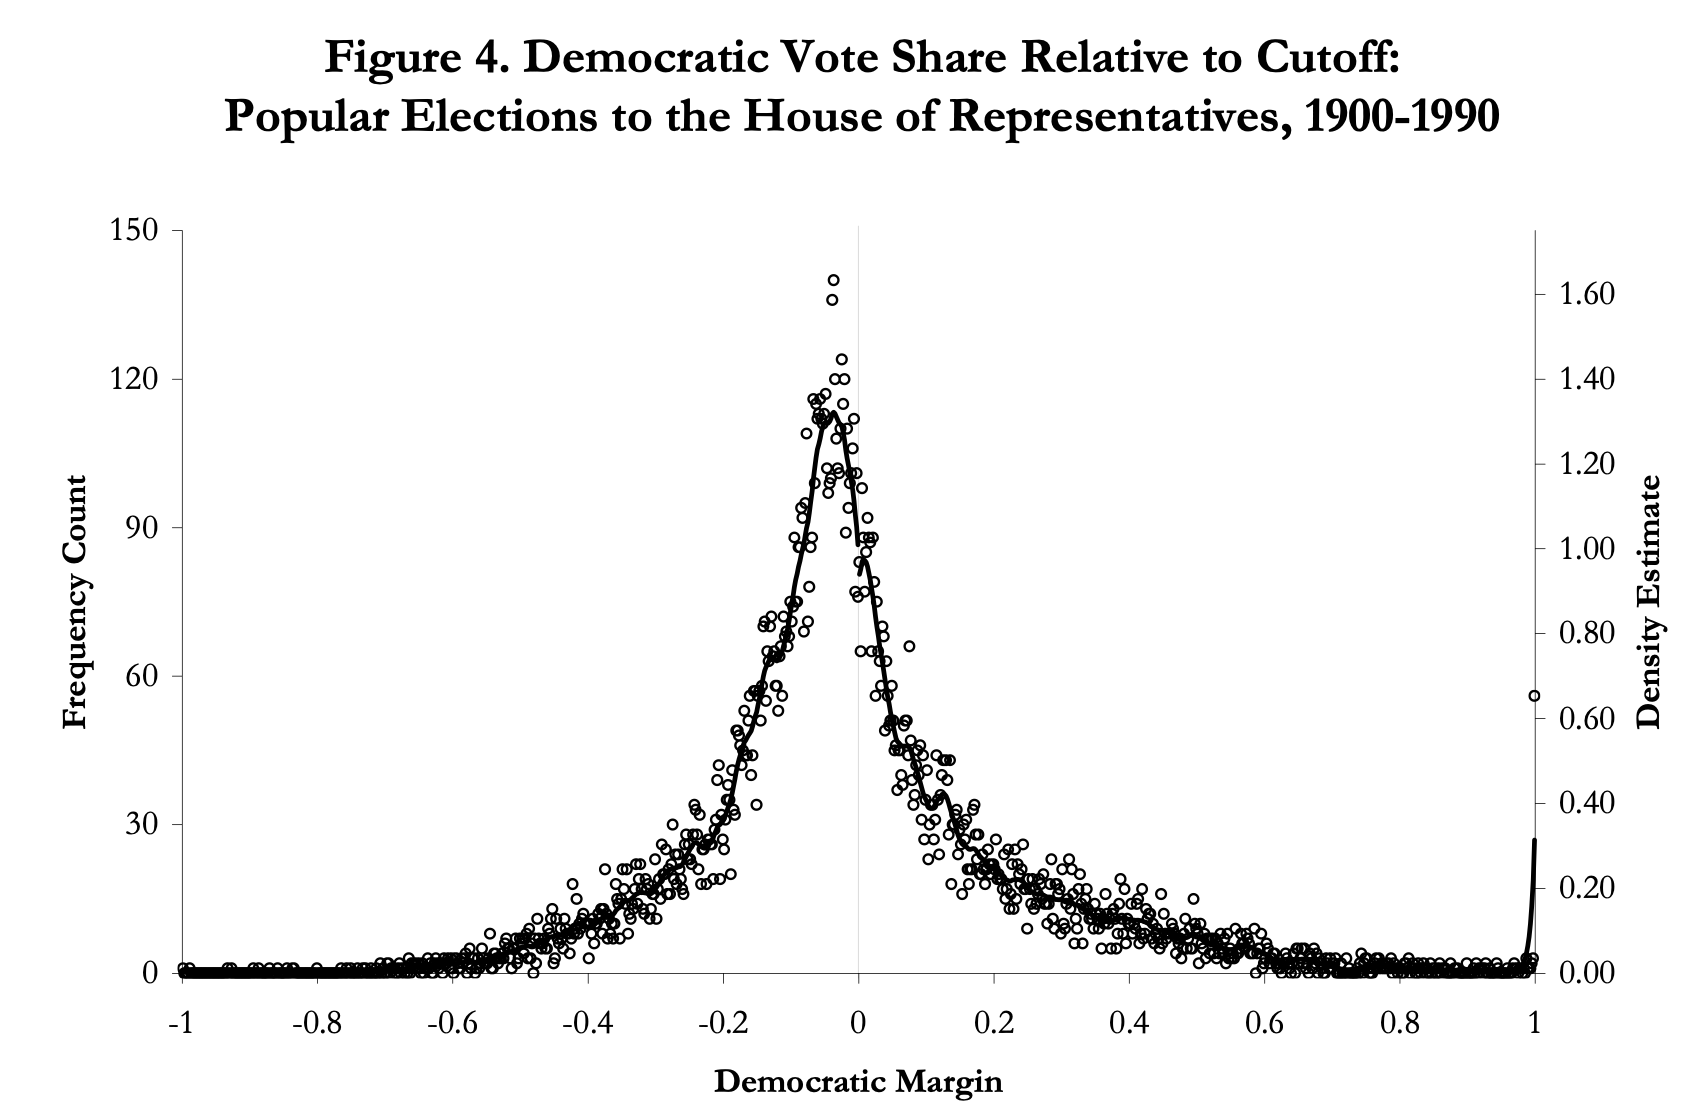
\includegraphics[height=0.9\textheight]{./resources/mccrary2.png}
\end{center}
\end{frame}


\begin{frame}{Manipulation: Bad}
\begin{center}
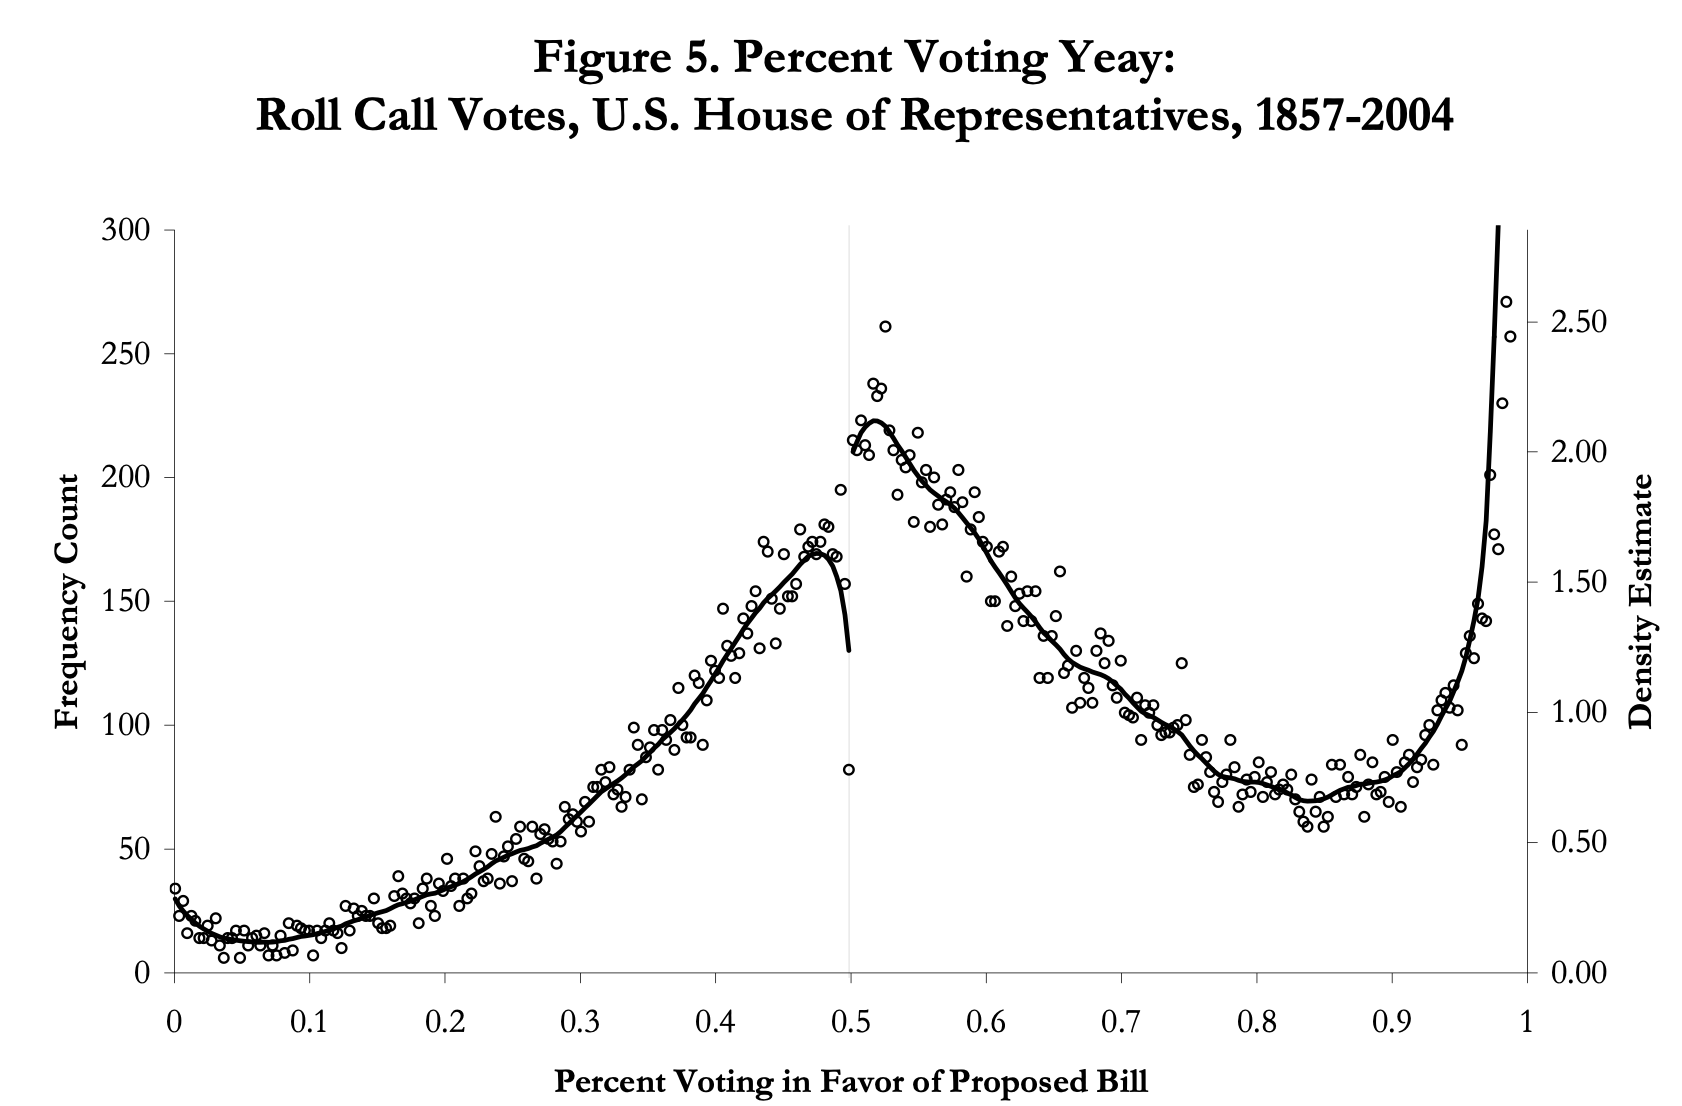
\includegraphics[height=0.9\textheight]{./resources/mccrary3.png}
\end{center}
\end{frame}

\section{Extensions}
\begin{frame}{Fuzzy RD}
\small 
An important extension in the \alert{Fuzzy RD}.   Back to where we started:
\begin{eqnarray*}
\lim_{x\rightarrow c^{+}} P(T_i | X_i = x) \neq \lim_{x\rightarrow c^{-}}P(T_i | X_i = x)
\end{eqnarray*}
\begin{itemize}
\item We need a discontinuous jump in probability of treatment, but it doesn't need to be $0 \rightarrow 1$.
\begin{eqnarray*}
\tau_i(c) = \frac{\lim_{x\rightarrow c^{+}} P(Y_i | X_i = x) - \lim_{x\rightarrow c^{-}}P(Y_i | X_i = x)}{\lim_{x\rightarrow c^{+}} P(T_i | X_i = x) - \lim_{x\rightarrow c^{-}}P(T_i | X_i = x)}
\quad \text{ Wald Estimator}
\end{eqnarray*}
\item Under sharp RD everyone was a \alert{complier}, now we have some \alert{always takers} and some \alert{never takers} too.
\item Now we are estimating the treatment effect only for the population of compliers at $x=c$.
\item This should start to look familiar. We are going to do IV!
\end{itemize}
\end{frame}

\begin{frame}{Related Idea: Kinks}
 A related idea is that of \alert{kinks}. 
\begin{itemize}
\item Instead of a discontinuous jump in the outcome there is a discontinuous jump in $\beta_i$ on $x_i$.
\item Often things like tax schedules or government benefits have a kinked pattern.
\end{itemize}
\end{frame}

\section{What about binscatter?}

\begin{frame}{Binscatter: Easy Version}
All of these RDD plots used something called \alert{binscatter}
\begin{itemize}
\item For the running variable $x_i$ break it up into $J=20,50,100$ bins of equal \alert{density}
\item Use the \alert{quantiles} of $x_i$.
\begin{itemize}
\item If we have 10 bins, each contains 10\% of the sample
\item Like a histogram but with \alert{bins of different width}.
\end{itemize}
\item Compute the average value:  $b_x^j=E[x_i | x_i \in \text{bin}_j]$
\item Compute the average value:  $b_y^j=E[y_i | x_i \in \text{bin}_j]$
\item Plot $(b_y^j,b_x^j)$ for each bin $j$.
\item Often draw a line of best fit through the points
\end{itemize}
But often we have other covariates!
\end{frame}


\begin{frame}{Binscatter: Under the Hood}
\begin{center}
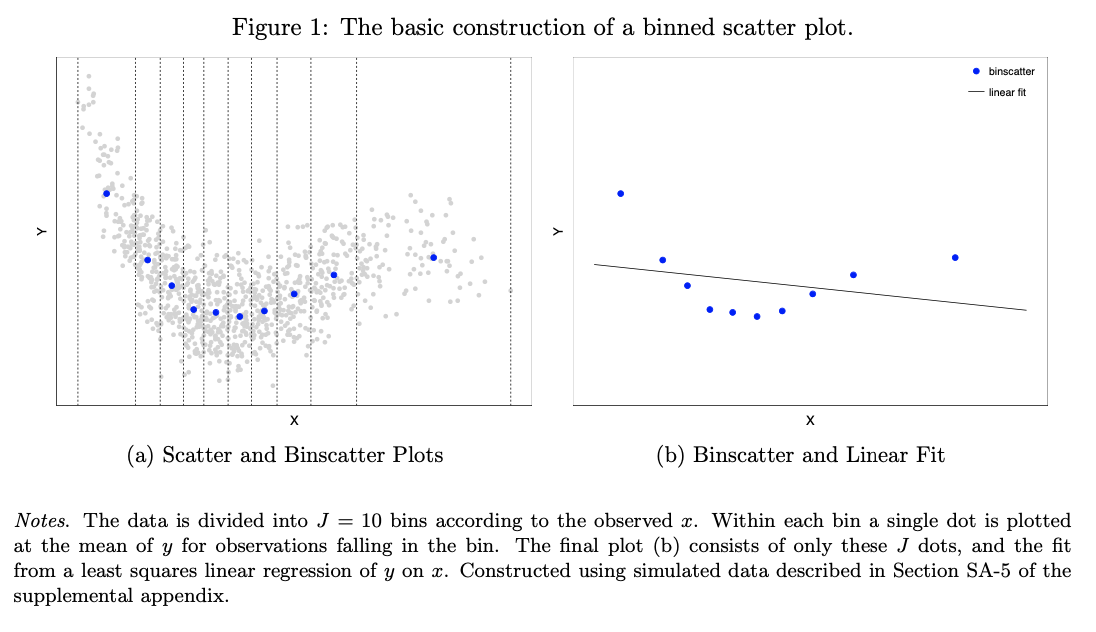
\includegraphics[height=0.9\textheight]{./resources/bs2.png}
\end{center}
\end{frame}


\begin{frame}{Binscatter: Under the Hood}
\begin{center}
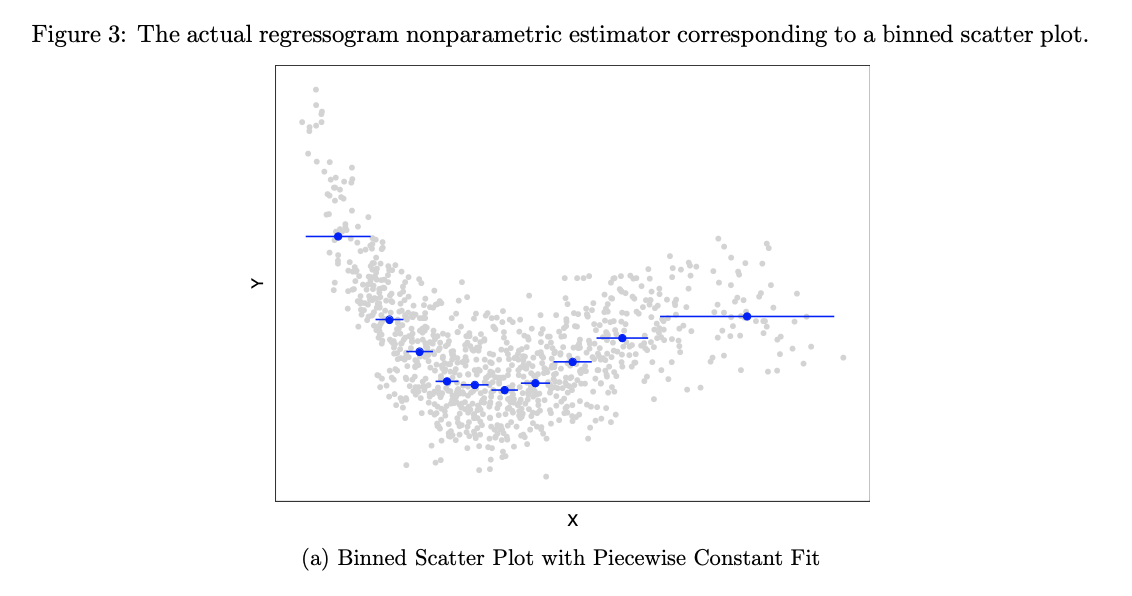
\includegraphics[height=0.9\textheight]{./resources/bs1.png}
\end{center}
\end{frame}


\begin{frame}{Binscatter as Semiparametric Regression:\\
\small Cattaneo, Crump, Farrell, Feng (2019)}
The right way to think of binscatter is as \alert{semiparametric} or \alert{partially linear} regression
\begin{align*}
y_{i}=\mu\left(x_{i}\right)+\mathbf{w}_{i}^{\prime} \gamma+\epsilon_{i}, \quad \mathbb{E}\left[\epsilon_{i} | x_{i}, \mathbf{w}_{i}\right]=0
\end{align*}
\begin{itemize}
\item Unless $u(x_i)$ is linear, we can't partial out $y_i -\mathbf{w}_{i}^{\prime} \gamma$ via Frisch-Lovell-Waugh
\item Most binscatter software does this wrong. Use \texttt{binsreg} in R.
\end{itemize}
\end{frame}

\section{Thanks}


%\begin{frame}{One quantity to rule them all: MTE}
%Heckman and Vytlacil provide a unifying non-parametric framework to categorize treatment effects. Their approach is known as the \alert{marginal treatment effect} or MTE
%\begin{itemize}
%\item The MTE isn't a number it is a \alert{function}.
%\item All of the other objects (LATE, ATE, ATT, etc.) can be written as integrals (weighted averages) of the MTE.
%\item The idea is to bridge the treatment effect parameters (stuff we get from running regressions) and the structural parameters: features of $f(\beta_i)$.
%\end{itemize}
%\end{frame}



\end{document}

